\section{无向树}
\begin{definition}
%@see: 《离散数学》(邓辉文) P198 定义7-3
不含有圈的连通无向图,称为\DefineConcept{无向树}(tree),简称为\DefineConcept{树}.
\end{definition}

含有\(n\ (n\geq1)\)个顶点的树,称为 \DefineConcept{\(n\)阶树}.
不含顶点的树,称为\DefineConcept{空树}.

\begin{property}
%@see: 《离散数学》(邓辉文) P199 性质1
\(n\ (n\geq1)\)阶树恰有\(n-1\)条边.
%TODO proof
\end{property}

\begin{property}
%@see: 《离散数学》(邓辉文) P199 性质2
\(n\ (n\geq2)\)阶树至少有2个度为\(1\)的顶点.
%TODO proof
\end{property}

\begin{theorem}
%@see: 《离散数学》(邓辉文) P199 定理7-8
设\(G = (V,E)\)是\((n,m)\)无向图,
则\begin{align*}
	&\text{$G$是一棵树} \\
	&\iff \text{$G$不含有圈} \quad\land\quad m=n-1 \\
	&\iff \text{$G$是连通图} \quad\land\quad m=n-1 \\
	&\iff \text{$G$不含有圈,但新增一条边后成为一个圈} \\
	&\iff \text{$G$是连通图,但删除任意一条边后成为非连通图} \\
	&\iff \text{$G$的每一对顶点有且仅有一条路径}.
\end{align*}
%TODO proof
\end{theorem}

\begin{definition}
%@see: 《离散数学》(邓辉文) P200 定义7-4
设\(G = (V,E)\)是无向图.
若\(G\)的生成子图\(T\)是树,
则称“\(T\)是\(G\)的\DefineConcept{生成树}(spanning tree)”.
\end{definition}

\cref{figure:图论.生成树.无向图1} 所示的无向图不是树,
但它的生成子图 \labelcref{figure:图论.生成树.无向图1的生成树1,figure:图论.生成树.无向图1的生成树2} 是树.

\begin{figure}[hbt]
%@see: 《离散数学》(邓辉文) P200 图7-21
	\centering
	\def\subwidth{.3\linewidth}
	\begin{subfigure}[b]{\subwidth}
		\centering
		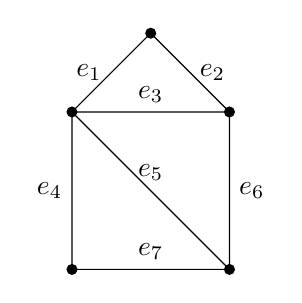
\begin{tikzpicture}
			\fill(0,0)coordinate(v1)circle(2pt);
			\fill(2,0)coordinate(v2)circle(2pt);
			\fill(2,2)coordinate(v3)circle(2pt);
			\fill(1,3)coordinate(v4)circle(2pt);
			\fill(0,2)coordinate(v5)circle(2pt);
			\draw(v3)--(v4)node[midway,right]{$e_2$}
				--(v5)node[midway,left]{$e_1$}
				--(v1)node[midway,left]{$e_4$}
				--(v2)node[midway,above]{$e_7$}
				--(v3)node[midway,right]{$e_6$}
				--(v5)node[midway,above]{$e_3$}
				--(v2)node[midway,above]{$e_5$};
		\end{tikzpicture}
		\caption{}
		\label{figure:图论.生成树.无向图1}
	\end{subfigure}~\begin{subfigure}[b]{\subwidth}
		\centering
		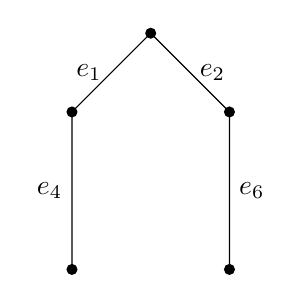
\begin{tikzpicture}
			\fill(0,0)coordinate(v1)circle(2pt);
			\fill(2,0)coordinate(v2)circle(2pt);
			\fill(2,2)coordinate(v3)circle(2pt);
			\fill(1,3)coordinate(v4)circle(2pt);
			\fill(0,2)coordinate(v5)circle(2pt);
			\draw(v2)--(v3)node[midway,right]{$e_6$}
				--(v4)node[midway,right]{$e_2$}
				--(v5)node[midway,left]{$e_1$}
				--(v1)node[midway,left]{$e_4$};
		\end{tikzpicture}
		\caption{}
		\label{figure:图论.生成树.无向图1的生成树1}
	\end{subfigure}~\begin{subfigure}[b]{\subwidth}
		\centering
		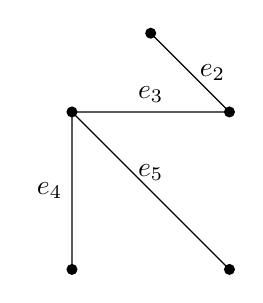
\begin{tikzpicture}
			\fill(0,0)coordinate(v1)circle(2pt);
			\fill(2,0)coordinate(v2)circle(2pt);
			\fill(2,2)coordinate(v3)circle(2pt);
			\fill(1,3)coordinate(v4)circle(2pt);
			\fill(0,2)coordinate(v5)circle(2pt);
			\draw(v4)--(v3)node[midway,right]{$e_2$}
				--(v5)node[midway,above]{$e_3$}
				--(v1)node[midway,left]{$e_4$}
				(v5)--(v2)node[midway,above]{$e_5$};
		\end{tikzpicture}
		\caption{}
		\label{figure:图论.生成树.无向图1的生成树2}
	\end{subfigure}
	\caption{}
\end{figure}

不是每一个无向图都有生成树.
即便某个无向图有生成树,它的生成树也不一定唯一.

\begin{theorem}
%@see: 《离散数学》(邓辉文) P201 定理7-9
设\(G\)是无向图,
则\(G\)有生成树的充分必要条件是\(G\)是连通图.
%TODO proof
\end{theorem}

\begin{corollary}
%@see: 《离散数学》(邓辉文) P201 推论
\(n\ (n\geq1)\)阶连通图至少有\(n-1\)条边.
\end{corollary}

\begin{corollary}
%@see: 《离散数学》(邓辉文) P201
\(n\ (n\geq1)\)阶树是边数最少的连通无向图.
\end{corollary}

\begin{example}
%@see: 《离散数学》(邓辉文) P201 例7-8
设\(G\)是连通无向图,
\(T\)是\(G\)的任意一棵生成树,
\(C\)是\(G\)的任意圈,
则\(C\)至少含有一条关于生成树\(T\)中的弦.
%TODO 什么是弦???未定义!
%TODO proof
\end{example}

\begin{example}
%@see: 《离散数学》(邓辉文) P201 例7-9
设\(G\)是连通无向图,
\(T\)是\(G\)的任意一棵生成树,
\(F\)是\(G\)的任意一个边割集,
则\(F\)至少有一条\(T\)中的树枝.
%TODO 什么是树枝???未定义!
%TODO proof
\end{example}

\begin{definition}
%@see: 《离散数学》(邓辉文) P201 定义7-5
设\(G\)是一个边赋权的连通无向图,
\(G\)的生成树\(T\)的各边的权之和,
称为“\(T\)的\DefineConcept{权}”.
\(G\)的权最小的生成树,
称为“\(G\)的\DefineConcept{最小生成树}(minimal spanning tree)”.
\end{definition}
